% -*- TeX:UK -*-
\documentclass[10pt]{beamer}
\usetheme{metropolis}
%\useinnertheme{rectangles}
\setbeamercovered{%
still covered={\opaqueness<1->{15}},
again covered={\opaqueness<1->{40}}}

\hypersetup{colorlinks,linkcolor=black,urlcolor=brown,citecolor=brown}

\usepackage{amsmath,amssymb,amsthm}
\usepackage{unicode-math}

% We set the Lucida OTF fonts as default
\usepackage{fontspec}
\setmainfont{Lucida Bright OT}
\setsansfont{Lucida Sans OT}
\setmonofont{Lucida Console DK}[Scale=MatchLowercase]

\newfontfamily\webglyphsfont{WebHostingHub-Glyphs}[Scale=0.7]
\newcommand\webglyphs[1]{{\webglyphsfont\symbol{#1}}}
\newcommand\Discussion{\colorbox{white}{\textcolor{black}{\webglyphs{"F134}}}\xspace}
\newcommand\DiscussionI{\colorbox{black}{\textcolor{white}{\webglyphs{"F134}}}\xspace}
\newcommand\DExamples{\colorbox{black}{\textcolor{white}{\webglyphs{"F134} examples?}}}
\newcommand\Reading{\colorbox{black}{\textcolor{white}{\webglyphs{"F0C1}}}\xspace}
\newcommand\ReadingI{\colorbox{white}{\textcolor{black}{\webglyphs{"F0C1}}}\xspace}
\newcommand\Video{\colorbox{white}{\textcolor{black}{\webglyphs{"F03D}}}\xspace}
\newcommand\Attention{\colorbox{black}{\textcolor{orange}{\webglyphs{"F05A}}}\xspace}
\newcommand\HomeWork{\colorbox{white}{\textcolor{black}{\webglyphs{"F5ED}}}\xspace}
\newcommand\HomeWorkI{\colorbox{black}{\textcolor{white}{\webglyphs{"F5ED}}}\xspace}
\newcommand\Advanced{\colorbox{black}{\textcolor{white}{\webglyphs{"F235}}}\xspace}

\newfontfamily\lineabasicfont{linea-basic-10}
\newcommand\basicicons[1]{{\lineabasicfont\symbol{#1}}}
\newcommand\timeforwards{\basicicons{"0079}}
\newcommand\timebackwards{\basicicons{"0064}}

\newfontfamily\lineaweatherfont{linea-weather-10}
\newcommand\weathericons[1]{{\lineaweatherfont\symbol{#1}}}
\newcommand\meteosun{\weathericons{"E038}}
\newcommand\meteosuncloud{\weathericons{"E042}}
\newcommand\meteorain{\weathericons{"E033}}
\newcommand\meteowind{\weathericons{"E054}}

\newfontfamily\uleaffont{Mini Pics Uprooted Leaf}
\newcommand\uleafmpics[1]{{\uleaffont\symbol{#1}}}
\newcommand\lowplants{\uleafmpics{"00CE}}
\newcommand\mediumplant{\uleafmpics{"006A}}
\newcommand\bush{\uleafmpics{"0039}}
\newcommand\smallplant{\uleafmpics{"0030}}
\newcommand\seedling{\uleafmpics{"002F}}
\newcommand\floweringplant{\uleafmpics{"00CA}}

\newfontfamily\utwigfont{Mini Pics Uprooted Twig}
\newcommand\utwigmpics[1]{{\utwigfont\symbol{#1}}}
\newcommand\grassplant{\utwigmpics{"0033}}

\newfontfamily\uinsectfont{Insect Icons}
\newcommand\uinsect[1]{{\uinsectfont\symbol{#1}}}
\newcommand\bug{\uinsect{"006F}}

\usepackage{polyglossia}
\setdefaultlanguage[variant = british, ordinalmonthday = false]{english}

\usepackage[style=authoryear-comp,firstinits,sortcites,maxcitenames=2,%
    mincitenames=1,maxbibnames=10,minbibnames=10,uniquename=mininit,%
    uniquelist=minyear,sortfirstinits=true]{biblatex}
\addbibresource{../references/ecophys.bib}
\renewcommand{\bibfont}{\small}

\usepackage{abbrev}



\newcommand*{\Px}{\ensuremath{\mathrm{P}}\xspace}
\newcommand*{\Pxfr}{\ensuremath{\mathrm{P_{fr}}}\xspace}
\newcommand*{\Pxr}{\ensuremath{\mathrm{P_r}}\xspace}
\newcommand*{\Pxtot}{\ensuremath{\mathrm{P_{tot}}}\xspace}

%\newcommand*{\COtwo}{\ensuremath{\textrm{CO}_2}\xspace}

\newcommand*{\nEff}{{\scriptsize 0}\xspace}
\newcommand*{\pEff}{\ensuremath{+}\xspace}
\newcommand*{\mEff}{\ensuremath{-}\xspace}
\newcommand*{\uEff}{?\xspace}

\newcommand*{\myatop}[2]{\genfrac{}{}{0pt}{3}{#1}{#2}}

\begin{document}

\title{PBIO-141\\Sensory and Physiological Ecology\\of  Plants}
\subtitle{8: Photoreceptors and signalling}
\author{Pedro J. Aphalo}
\date{January--February 2022}
\institute[Univ.\ of Helsinki]{M.Sc.\ in Plant Biology, University of Helsinki\\[2ex] \url{http://blogs.helsinki.fi/aphalo/}}


  \begin{frame}
    \maketitle
  \end{frame}

  \begin{frame}[c]
    \begin{center}
      \begin{small}
        \copyright 2006--2022 by Pedro J. Aphalo\\
        University of Helsinki, Finland.\\
        \textcolor{blue}{\url{http://blogs.helsinki.fi/senpep-blog/}}\\[2ex]
      \end{small}

      \begin{footnotesize}
        Sensory and Physiological Ecology of Plants slides by Pedro J. Aphalo are licensed under a Creative Commons Attribution-ShareAlike 4.0 International License.

      
\includegraphics[width=6em]{../figures/copyright/by-sa}\\[2ex]
      \end{footnotesize}
        
        \begin{scriptsize}
        Typeset in Lucida Sans, \textrm{Luicda Bright}, \texttt{Lucida Console} and Lucida Math. Icons from fonts ``WebHostingHub Glyphs'' (under SIL-Open Font License) from \url{https://www.webhostinghub.com/}; ``insect icons'' (free from \url{http://www.woodcutter.es/}); ``linea-basic-10'' and ``linea-weather-10'' (free from \url{https://github.com/linea-io}), ``Mini Pics Uprooted Twig'' and ``Mini Pics Uprooted Twig'' (commercial, from Image Club Graphics, Inc.). Plant icon as .svg by Abdul Wahhab (free from \url{NounProject.com}).

        Illustrations and text quoted from copyrighted sources is excluded from this license and their use should respect the original licenses.
        \end{scriptsize}
    \end{center}
  \end{frame}


  \begin{frame}
    \frametitle{Outline}
    \tableofcontents
  \end{frame}

\section{The photoreceptors}

\begin{frame}{Phytochromes: Molecular configuration}
    \centering
    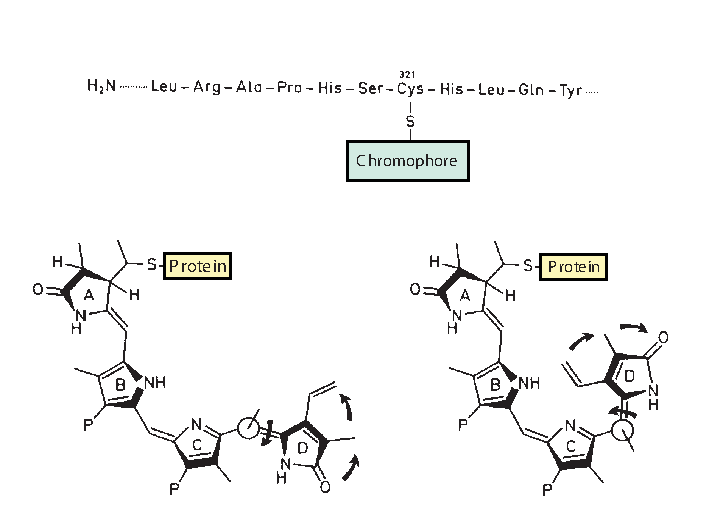
\includegraphics[width=0.9\textwidth]{../figures/P_structure_colour}\\
    {\small Left: P$_\mathrm{r}$, right: P$_\mathrm{fr}$ \autocite[from][]{Mohr1995}.}
\end{frame}

\begin{frame}{Phytochromes: Modes of action}
    \centering
    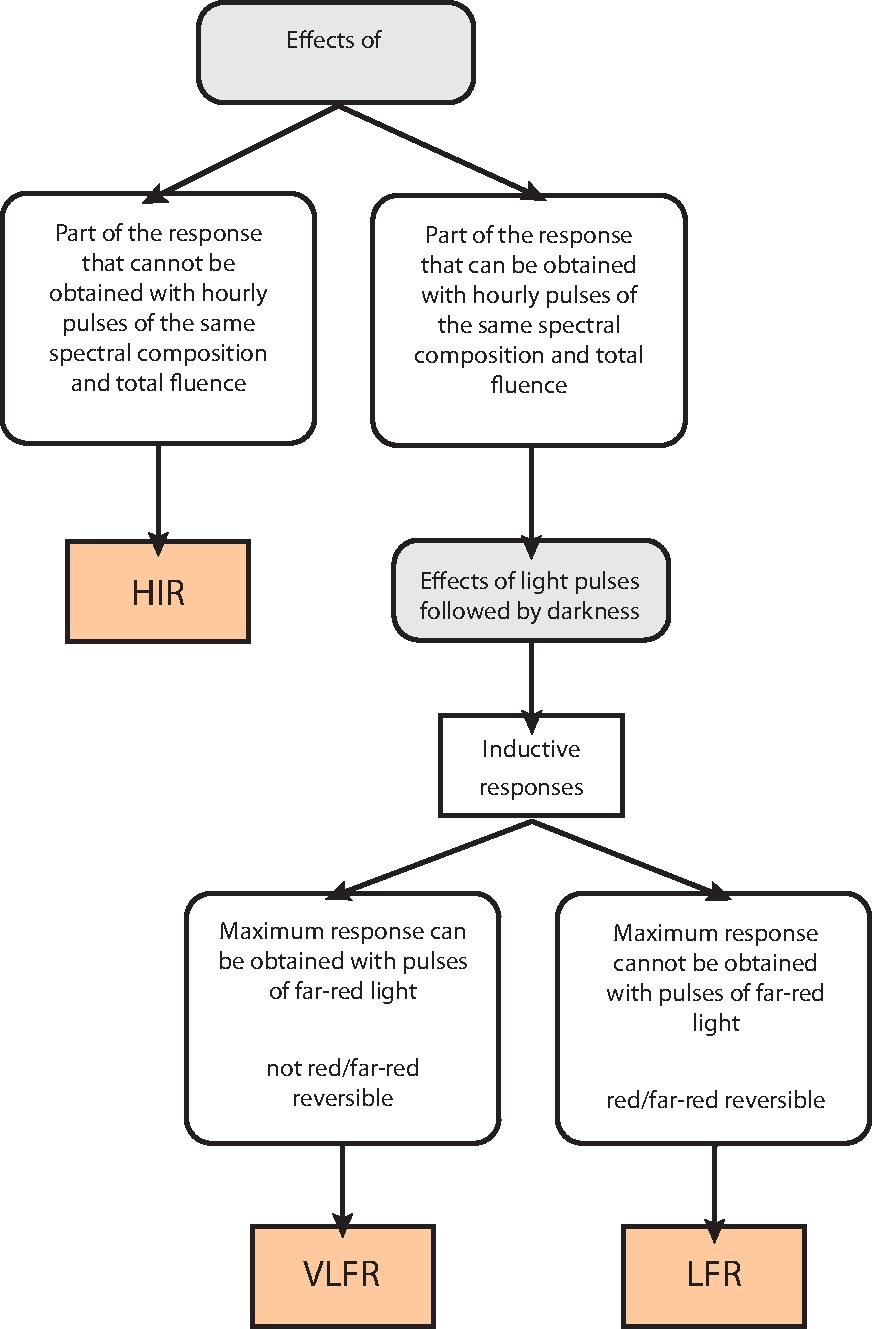
\includegraphics[height=0.85\textheight]{../figures/phytochrome_effects_c}
%    {\small Modes of action of phytochrome.}
\end{frame}

\begin{frame}{Photoreceptors: Typographical convention}
    \begin{description}
        \item Holoprotein (apoprotein + chromophore) $\rightarrow$ phyA
        \item Apoprotein $\rightarrow$ PHYA
        \item Gene $\rightarrow$ \textsl{PHYA}
        \item Mutant $\rightarrow$ \textsl{phyA}
    \end{description}
\end{frame}

\begin{frame}{Phytochromes: Phylogeny of apoprotein}
    \centering
    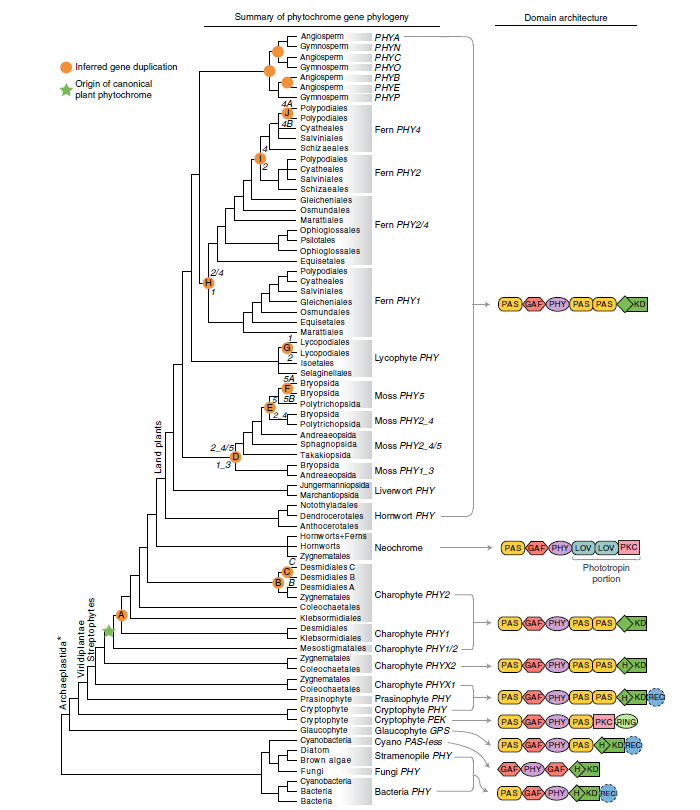
\includegraphics[height=0.9\textheight]{../figures/phy_phylogeny1}\\
    {\footnotesize \autocite[Fig.\ 1 in][]{Li2015}.}
\end{frame}

\begin{frame}{Phytochromes: Diversity and evolution of phytochrome}
    \centering
    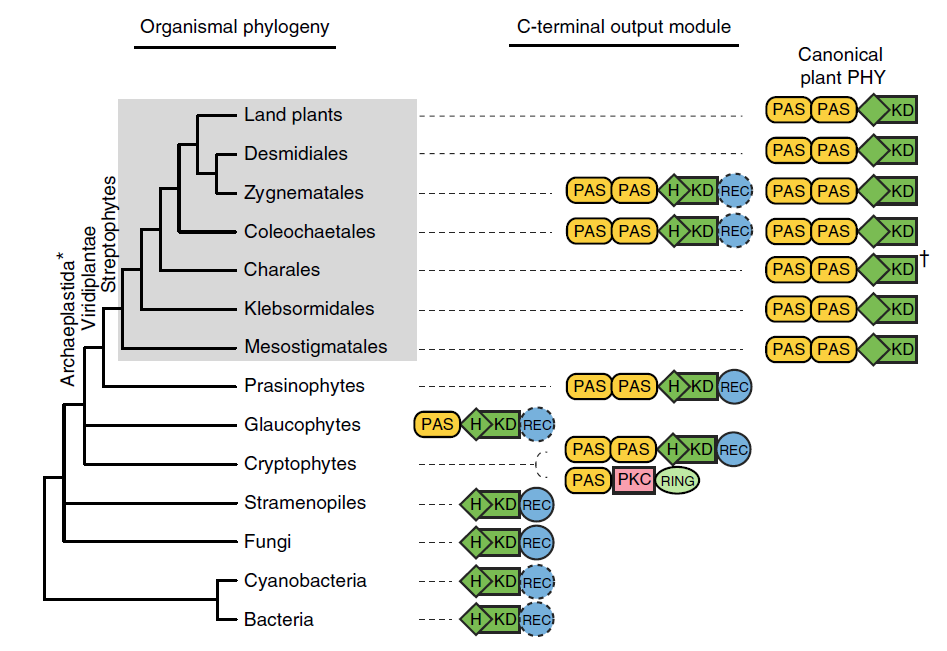
\includegraphics[height=0.8\textheight]{../figures/phy_phylogeny}\\
    {\footnotesize \autocite[Fig.\ 2 in][]{Li2015}.}
\end{frame}

\begin{frame}{Phytochromes}{Spectral tuning in algae}
    \centering
    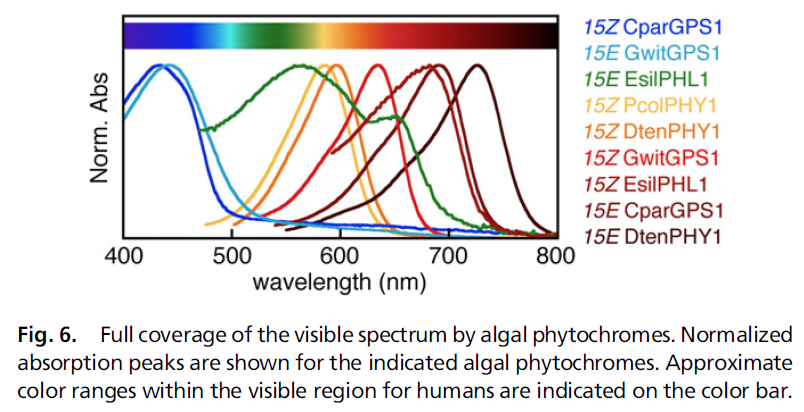
\includegraphics[height=0.7\textheight]{../figures/Rockwell2014_tuning6}\\
    {\footnotesize \autocite[Fig.\ 6 in][]{Rockwell2014}.}
\end{frame}

\begin{frame}{The photoreceptors: Blue/UV-A}
    \begin{itemize}
        \item Flavoproteins
        \begin{itemize}
            \item CRY1, CRY2 (FAD, flavin adenine dinucleotide + MTHF, methenyltetrahydrofolate)
            \item PHOT1, PHOT2, ZTL (FMN, flavin mononucleotide)
        \end{itemize}
        \item Carotenoid chromophore
        \begin{itemize}
            \item ? (zeaxanthin)
        \end{itemize}
    \end{itemize}
\end{frame}

\begin{frame}{Cryptochromes: structure}
    \centering
    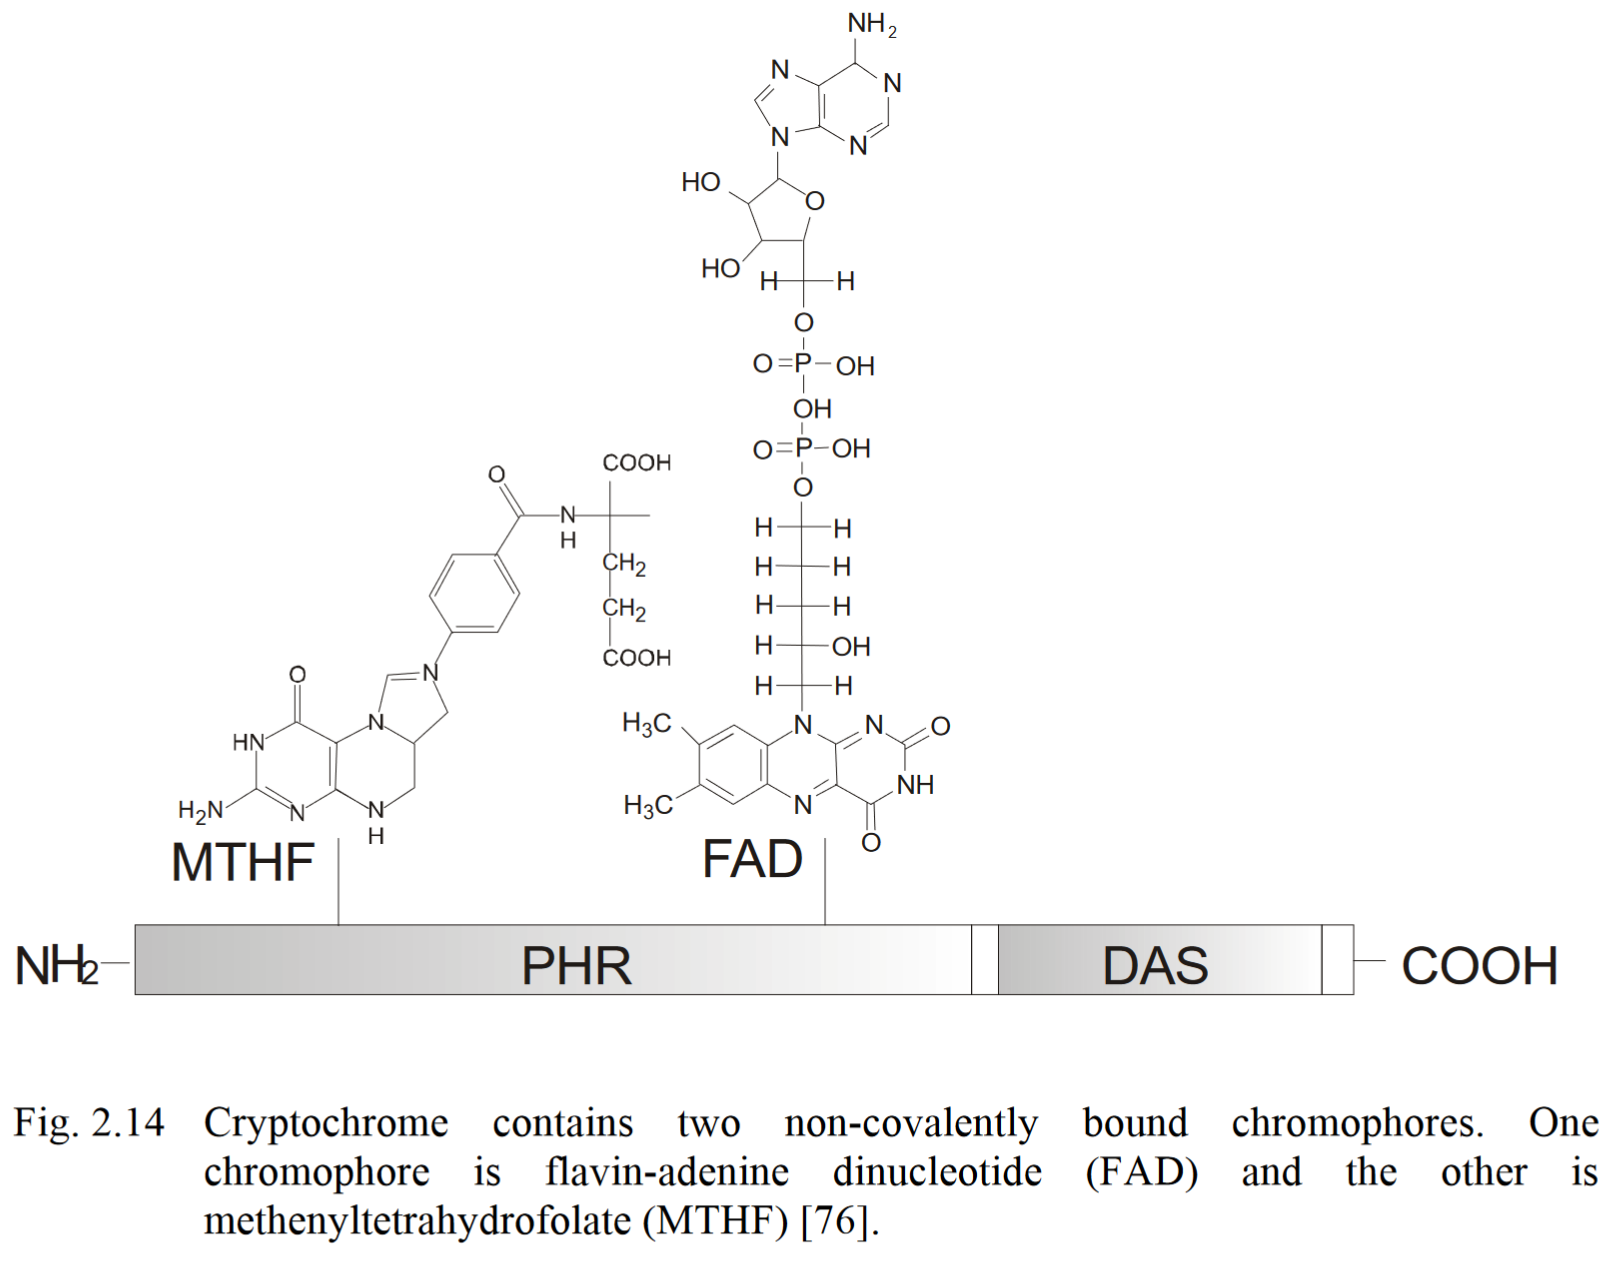
\includegraphics[height=0.9\textheight]{../figures/cryptochrome-Song-2006}\\
    {\footnotesize \autocite[from][]{Song2006}.}
\end{frame}

\begin{frame}{Cryptochromes (\emph{Arabidopsis thaliana})}
    \centering
    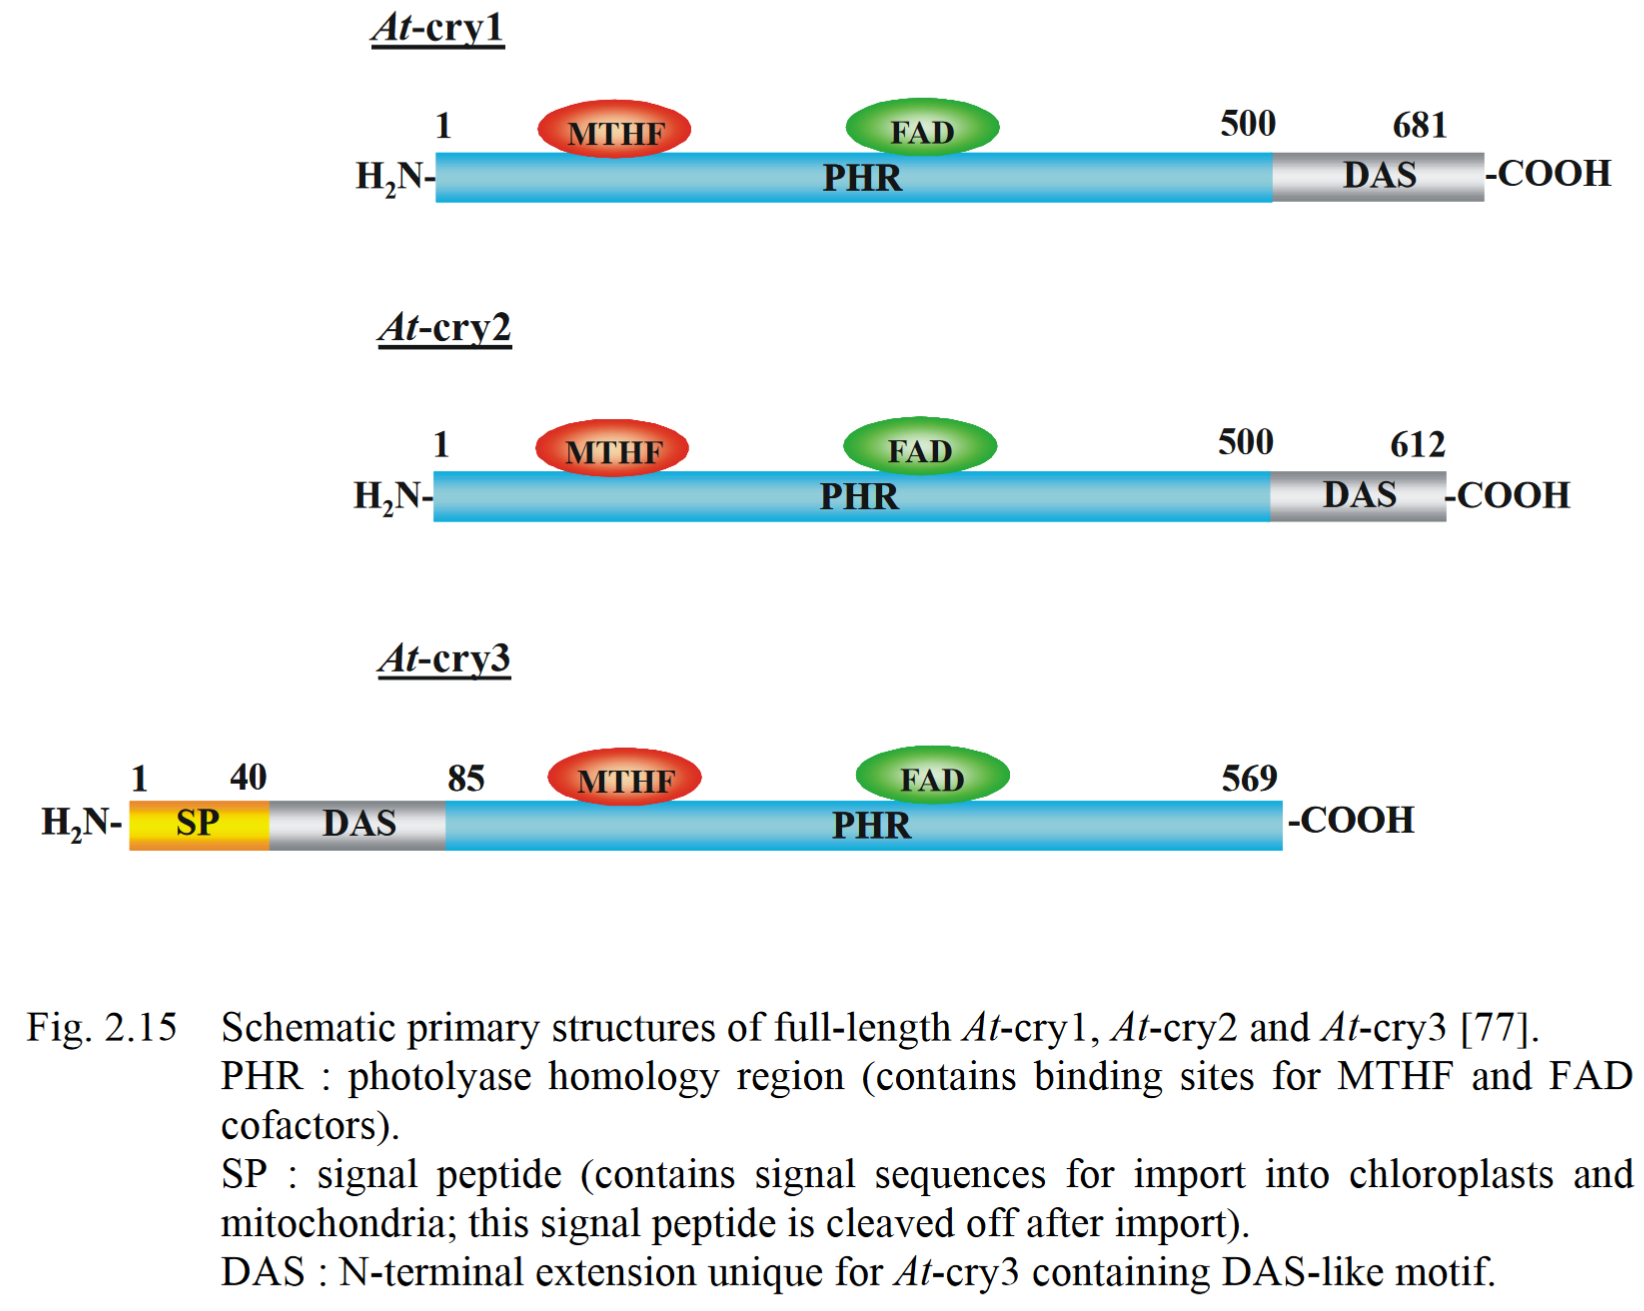
\includegraphics[height=0.8\textheight]{../figures/cryptochromes-At-Song-2006}\\
    {\footnotesize \autocite[from][]{Song2006}.}
\end{frame}

\begin{frame}{Phototropins: structure}
    \centering
    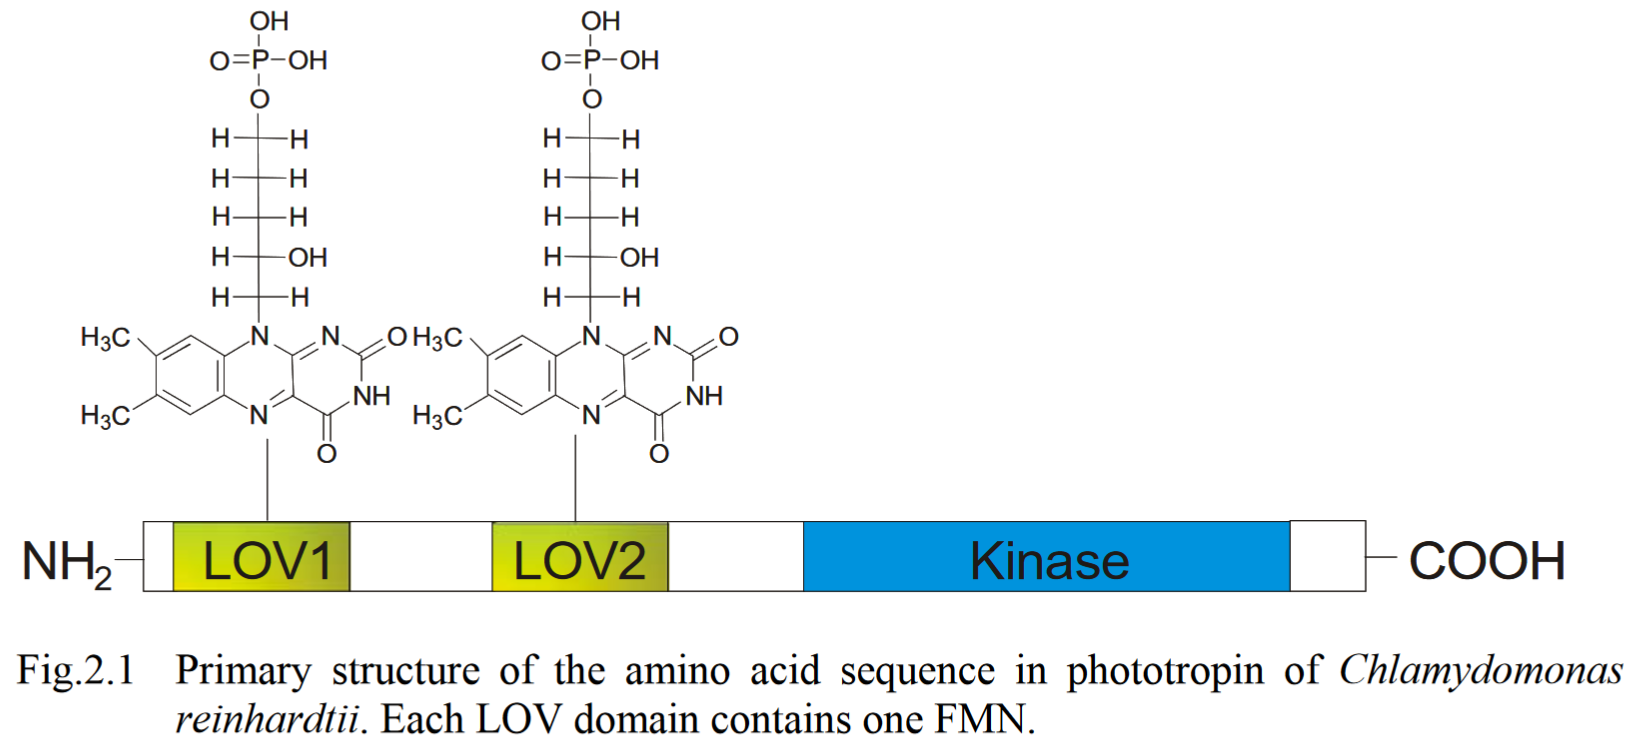
\includegraphics[width=0.9\textwidth]{../figures/phototropin-Song-2006}\\
    {\footnotesize \autocite[from][]{Song2006}.}
\end{frame}

\begin{frame}{Cryptochromes vs.\ phototropins}
    \begin{description}
        \item[Cryptochromes] `Slow responses to blue light': many responses.
        \item[Phototropins] `Movements': phototropism, stomatal opening, chloroplast movements.
        \item[Cryptochromes] plants, bacteria, fungi, animals, humans.
        \item[Phototropins] plants (also ferns, mosses, green algae)
        \item[Neochrome] Adiantum (fern). Phototropin fused to phy photosensory domain.
        \item[LOV proteins] plants, fungi, bacteria. Arabidopsis: ZTL/ADO family of blue photoreceptors.
    \end{description}
\end{frame}

\begin{frame}{The photoreceptors: UV-B}
    \begin{itemize}
        \item Photoreceptor: UVR8
        \item Responses:
        \begin{itemize}
            \item \textsl{CHS}: induction
            \item \textsl{Rbc S} (Rubisco small subunit): repression
            \item anthocyanin synthesis: \pEff
            \item some flavonoids: \pEff
            \item other flavonoids: \mEff $|$ \nEff
            \item stem elongation and other morphological effects
        \end{itemize}
    \end{itemize}

    Also damage is caused by UV-B, because it is absorbed
    by DNA and proteins.
\end{frame}

\begin{frame}{UVR8: structure}
    \centering
    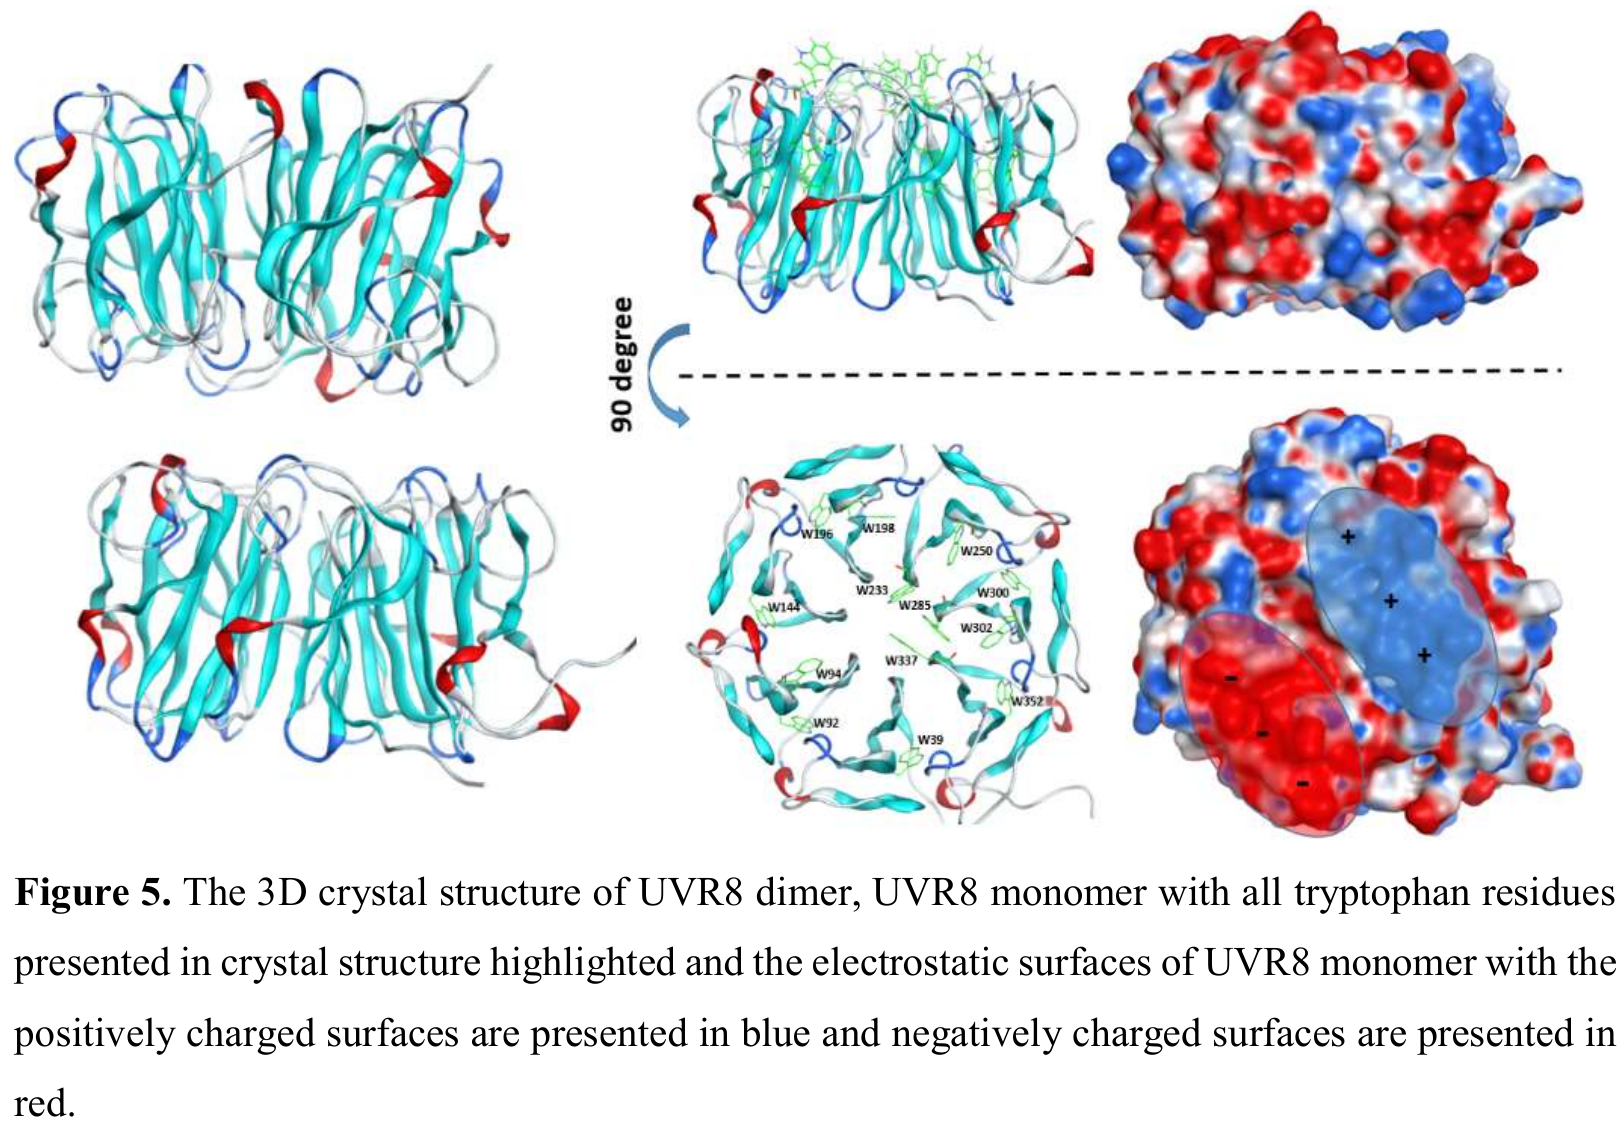
\includegraphics[width=0.9\textwidth]{../figures/UVR8-Wu2017}\\
    {\footnotesize \autocite[from][]{Wu2017}.}
\end{frame}

\section{Transduction}

\begin{frame}{Transduction: signalling networks}
    Cellular responses
    \begin{itemize}
        \item Gene transcription (up- or down regulation)
        \item Post-transcriptional regulation (e.g.\ enzyme activity)
        \item Post-transcriptional modification
        \item Membrane permeability (e.g.\ opening/closing of ion channels)
    \end{itemize}
\end{frame}

\begin{frame}{Cellular transduction chains}
    Transduction chains
    \begin{itemize}
        \item Complex interactions
        \item More like \textsl{webs} than \textsl{chains}
        \item<3-> Different for:
        \begin{itemize}
            \item different photoreceptors (even within families)
            \item different modes of action
            \item different end responses
            \item different tissues and developmental stages
        \end{itemize}
    \end{itemize}

    This complexity implies many possibilities for evolution and natural
    selection.
\end{frame}

\begin{frame}{Schematic model for phyA signalling}
    \centering
    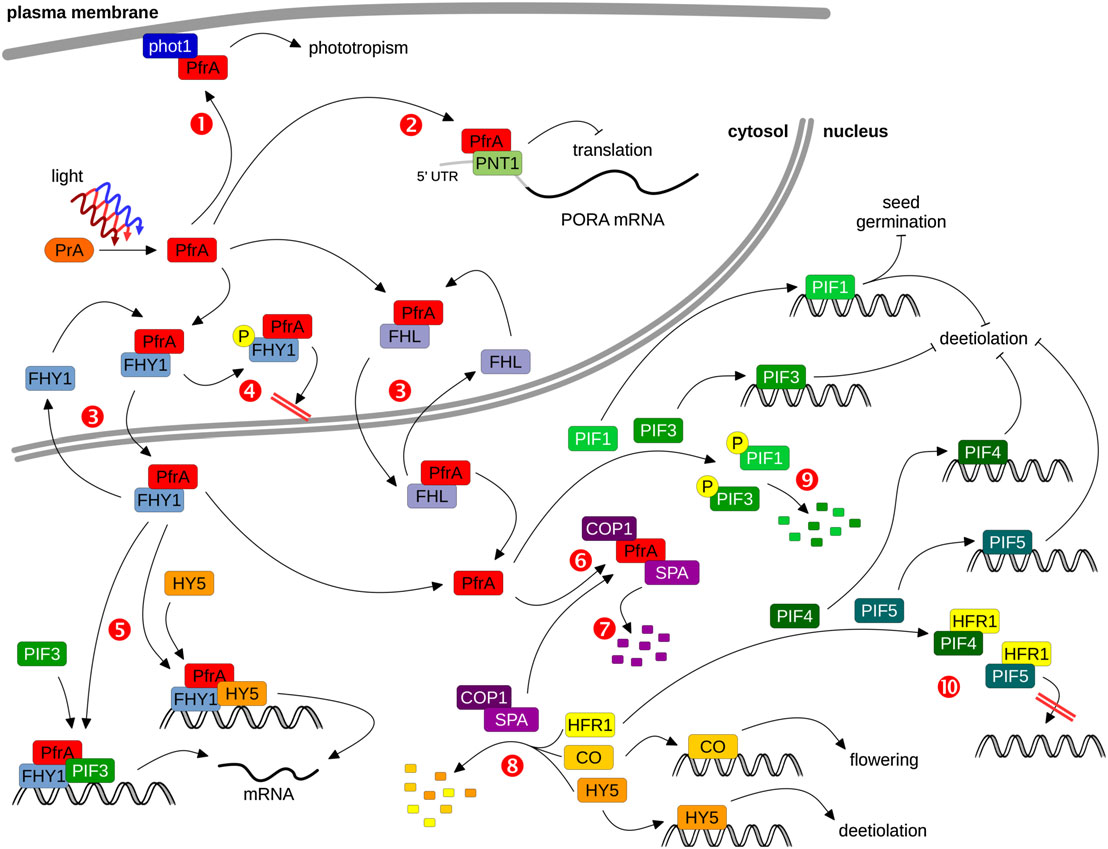
\includegraphics[height=0.85\textheight]{../figures/Sheerin2017-phyA-signalling-fig-only.jpg}\\
    {\footnotesize \autocite[Fig.\ 2 in][]{Sheerin2017}.}
\end{frame}

\begin{frame}{Schematic model for UVR8 and CRY signalling}
    \centering
    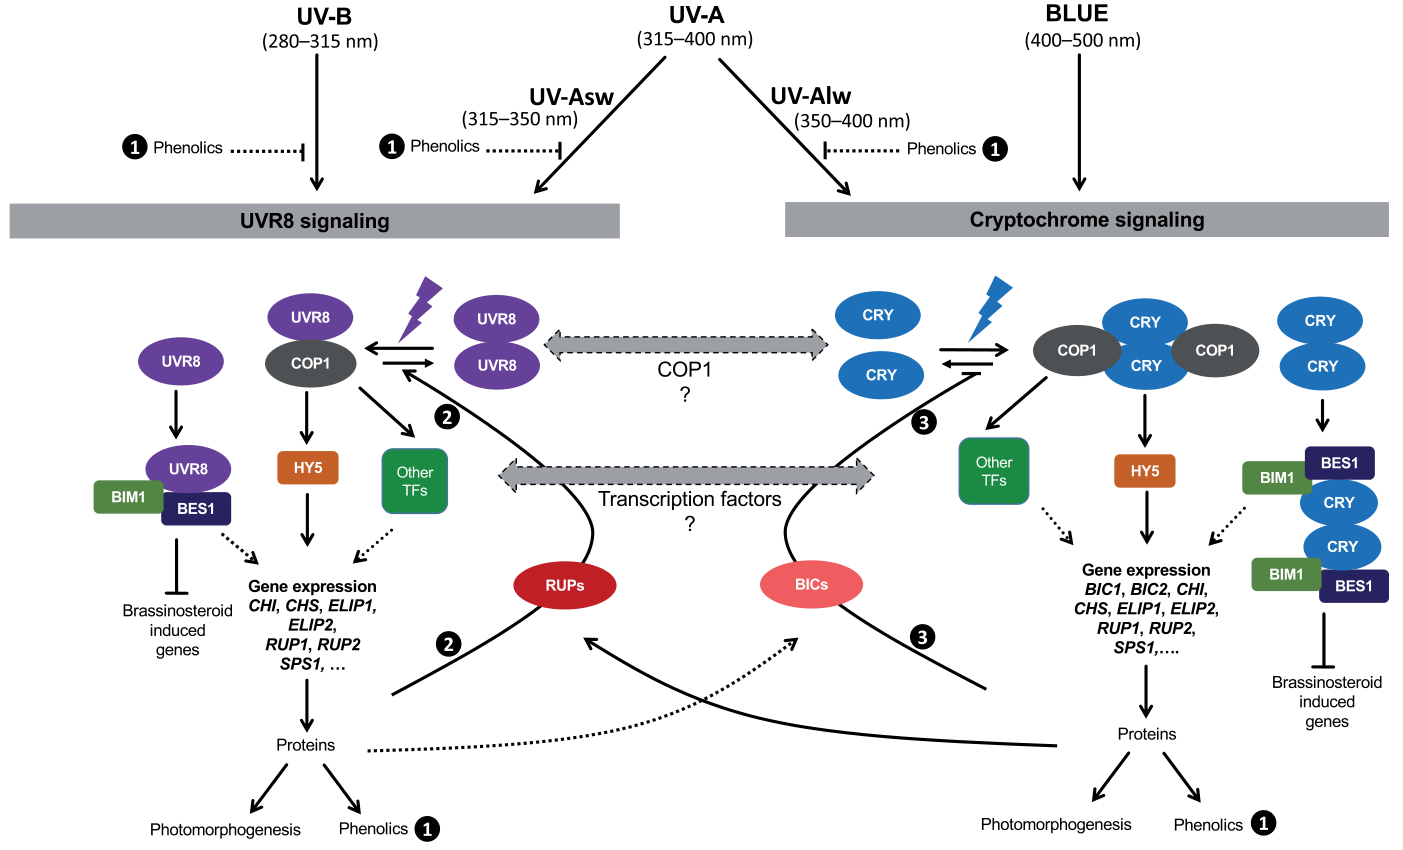
\includegraphics[width=0.95\textwidth]{../figures/Rai2021-fig5}\\
    {\footnotesize \autocite[Fig.\ 5 in][]{Rai2021}.}
\end{frame}

\begin{frame}{PIF signalling}
    \centering
    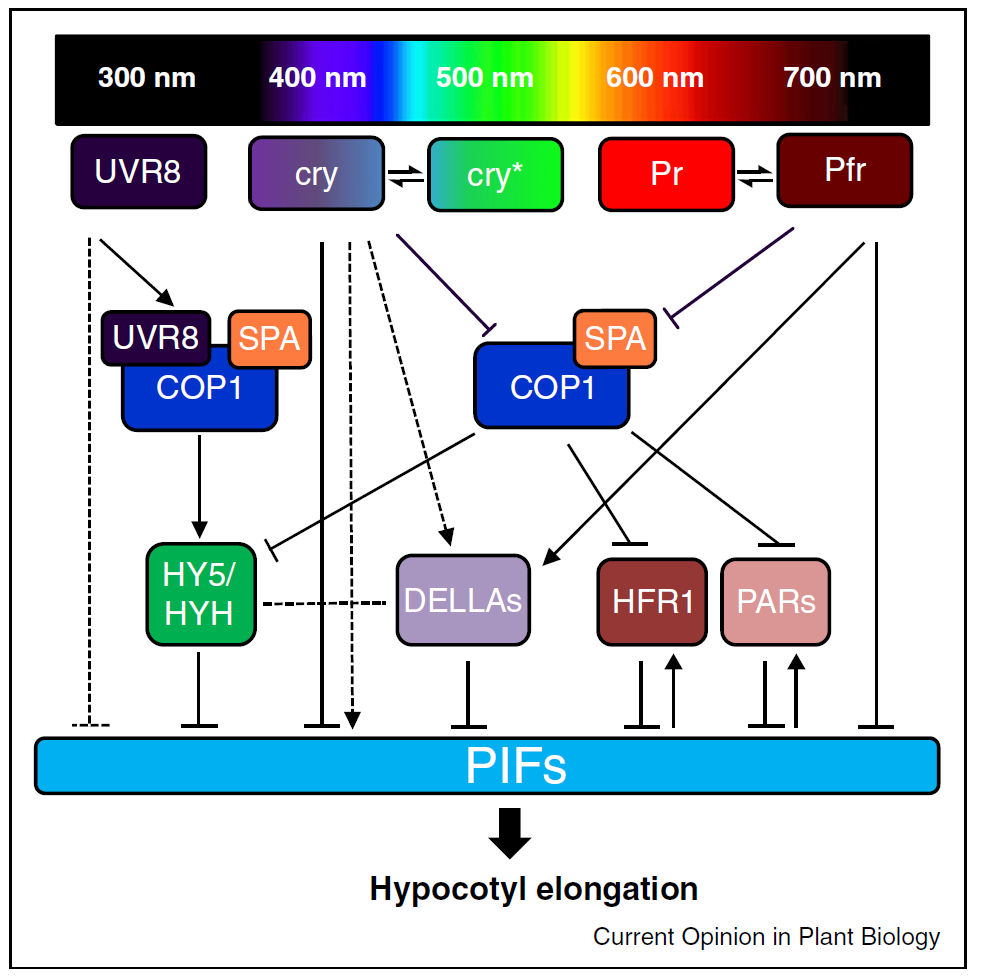
\includegraphics[height=0.85\textheight]{../figures/Fraser2016-PIF-signalling.png}\\
    {\footnotesize \autocite[Fig.\ 6 in][]{Fraser2016}.}
\end{frame}

\begin{frame}{HY5 signalling}
    \centering
    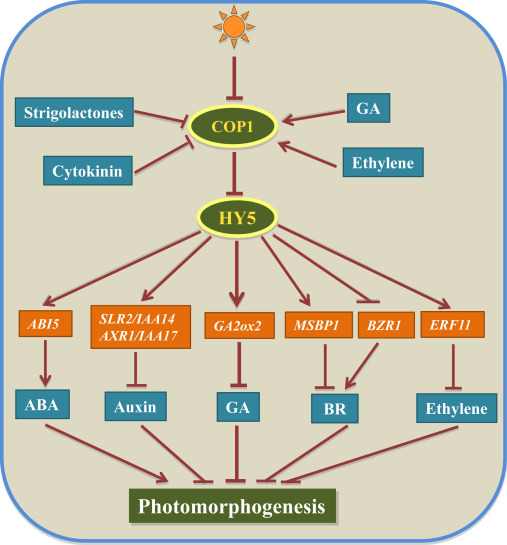
\includegraphics[width=0.4\textwidth]{../figures/Gangappa2016-HY5-hormones}%
    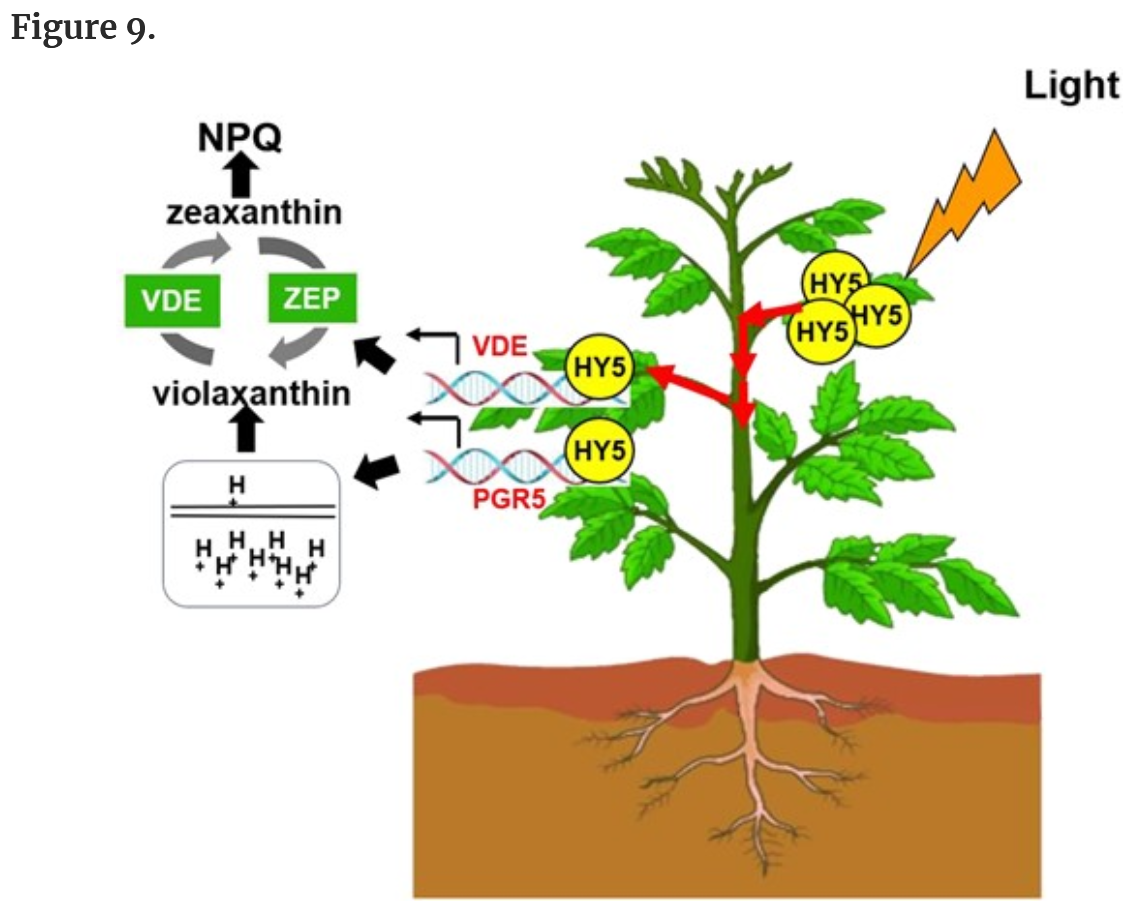
\includegraphics[width=0.57\textwidth]{../figures/Jiang2020-HY5}\\
    {\footnotesize \autocite[Fig.\ 6 in][]{Jiang2020a,Gangappa2016}.}
\end{frame}

\begin{frame}{Thermomorphogenesis}
    \centering
    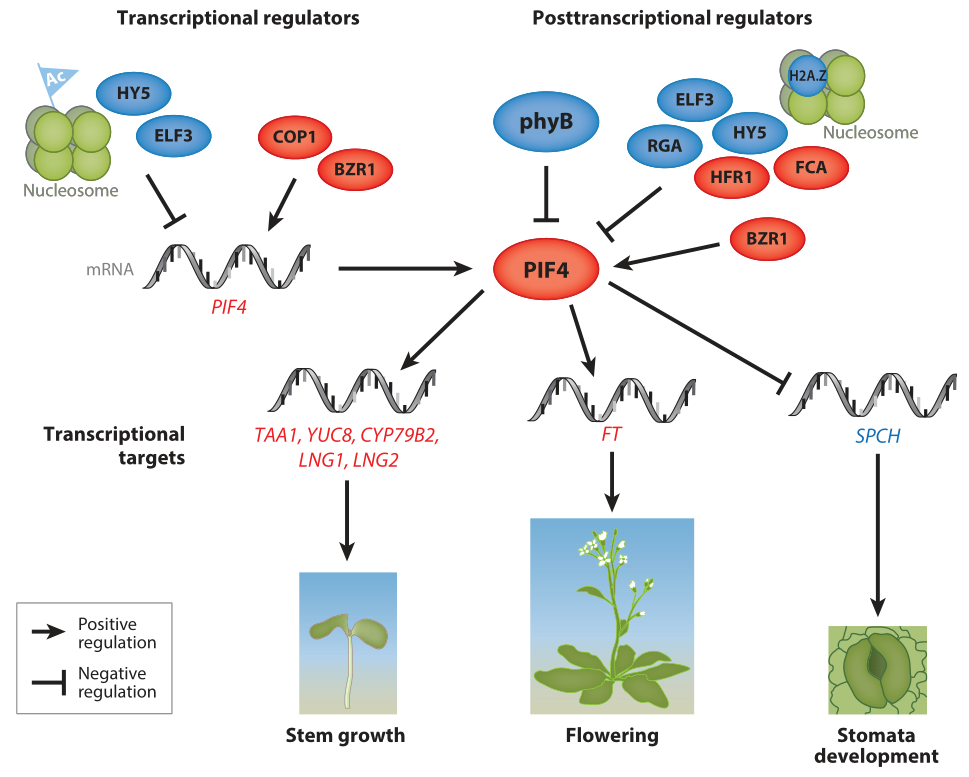
\includegraphics[height=0.85\textheight]{../figures/Casal2019-thermomorphogenesis}\\
    {\footnotesize \autocite[Fig.\ 6 in][]{Casal2019}.}
\end{frame}

\begin{frame}{Photosynthetic capacity: Transcription factor interaction network}
    \centering
    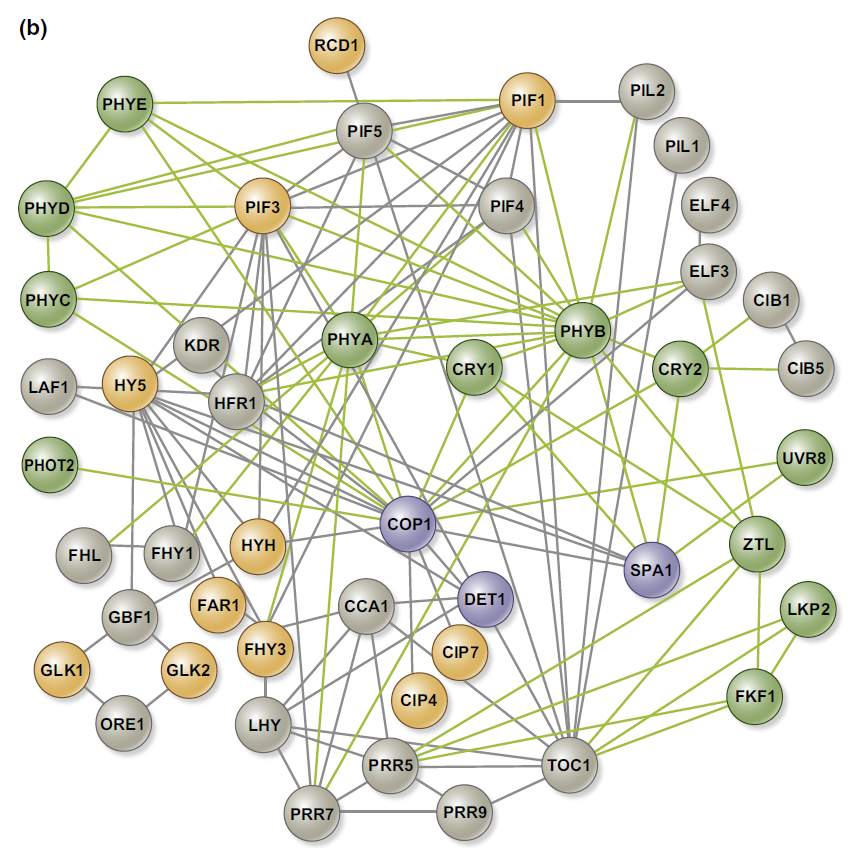
\includegraphics[height=0.8\textheight]{../figures/Wang2017b-fig2-b.png}\\
    {\footnotesize \autocite[Fig.\ 2 in][]{Wang2017b}.}
\end{frame}


  \section*{References}
  \begin{frame}[t,allowframebreaks]
    \frametitle{References}
    \printbibliography
  \end{frame}

\end{document}

\section{Whole plant responses to light cues}

\begin{frame}{Whole plant responses to light}
    \begin{itemize}
        \item Seed germination
        \item Size and shape of leaves
        \item Stem elongation in sparse canopies
        \item Regulation of metabolism of phenolics
    \end{itemize}
\end{frame}

\begin{frame}{Germination: Phytochrome-mediated responses}
    \begin{itemize}
        \item VLFR, LFR, HIR
        \item Embryo, other tissues
        \item LFR, normally FR: \mEff, R: \pEff
        \item VLFR, in buried seeds (tillage)
        \item HIR, continuous FR: \mEff
    \end{itemize}
\end{frame}

\begin{frame}{Leaf area expansion: Phytochrome-mediated responses}
    \begin{itemize}
        \item End-of-day light treatment
        \item Interaction with other responses affecting allocation
        \item Size
        \item Shape
        \item Number
        \item Consequences:
        \begin{itemize}
            \item light `harvesting' efficiency
            \item gas and energy exchange
        \end{itemize}
    \end{itemize}
\end{frame}


\begin{frame}{Phenolics: Anthocyanins}
\textbf{PHY-, CRY-, UVR8-mediated responses}
    \begin{itemize}
        \item Much studied: anthocyanin synthesis
        \item Induced by UV and VIS radiation
        \item Coarse regulation by induction of gene transcription
        \item Fine regulation by post-translational control
        \item Phytochrome could be the main effector
        \item Further regulation by blue/UV-A or UV-B
        \item Role of different photoreceptors is different in different species
        \item Further control by development stage or plant size
    \end{itemize}
\end{frame}

\begin{frame}{Phenolics: Flavonoids}
\textbf{PHY-, CRY-, UVR8-mediated responses}
    \begin{itemize}
        \item Multiple roles: UV-screens, anti-oxidants, biotic interactions
        \item Flavonoids frequently measured as absorbance at 300 nm in a crude extract
        \item Effect of UV-B is compound specific
        \item Secondary chemistry is very variable between individuals in a population
        \item Secondary chemistry is very variable among species
        \item Maximum absorbance at $\approx$ 360 to 375 nm.
    \end{itemize}
\end{frame}

\begin{frame}{Phenolics: Sinapates and other hydroxy-cinnamic acid derivatives}
    \begin{itemize}
        \item Possible multiple roles: UV-screens, anti-oxidants, biotic interactions
        \item Flavonoids frequently measured as absorbance at 300 nm in a crude extract
        \item Effect of UV-B is probably compound specific
        \item Secondary chemistry is very variable between individuals in a population
        \item Secondary chemistry is very variable among species
        \item Maximum absorbance in the UVB region.
    \end{itemize}
\end{frame}

%\begin{frame}{Albedo of vegetation}
%%    \vspace{-0.04\textheight}
%    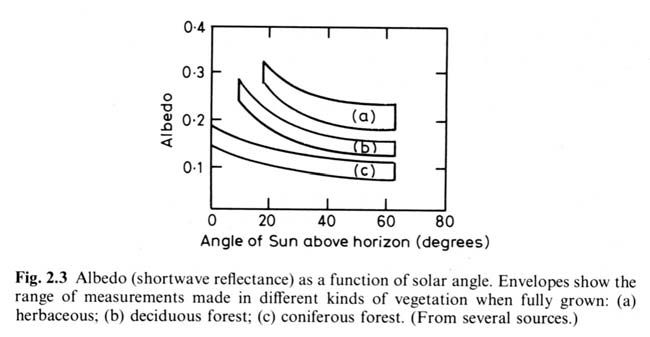
\includegraphics[width=\textwidth]{figures/Grace2.3Albedo.eps}\\
%    \vspace{-0.01\textheight}
%    {\small \citep[from][]{Grace1983}.}
%\end{frame}

%\begin{frame}{}
%    \vspace{-0.04\textheight}
%    \includegraphics[height=0.7\textheight]{figures/Willmer.eps}\\
%    \vspace{-0.01\textheight}
%    {\small \citep[from][]{WilFri1996}.}
%\end{frame}

%\begin{frame}{}
%    \vspace{-0.04\textheight}
%    \includegraphics[height=0.7\textheight]{figures/Taiz9.2CosineLaw.eps}\\
%    \vspace{-0.01\textheight}
%    {\small .}
%\end{frame}



%\begin{frame}{Cosine law}
%    \vspace{-0.07\textheight}
%    \twocolumn[lcolwidth=0.57\linewidth,rcolwidth=0.37\linewidth]{
%    \includegraphics[height=0.8\textheight]{figures/Taiz9.2CosineLaw.eps}}{%
%    \raggedright
%    \vspace{0.1\textheight}
%    {\small Irradiance on a surface depends on the angle of incidence
%    \citep[from][]{TaiZei2006}.}}
%\end{frame}

\section{Light cues and plant populations}

\begin{frame}{Light cues and populations:}
    \begin{itemize}
        \item Timing and location
        \item Searching for light
        \item Light, roots and mineral nutrients
        \item Being good neighbours
    \end{itemize}
\end{frame}

\begin{frame}{Light cues and populations: Timing and location}
    \begin{itemize}
        \item Hardening and de-hardening
        \item Flowering
        \item Germination
        \item De-etiolation
    \end{itemize}

    \begin{itemize}
        \item Synchronization of endogenous clock
        \item Phytochrome and cryptochrome
        \item Temperature
    \end{itemize}
\end{frame}

\begin{frame}{Light cues and populations: Searching for light}
    \begin{itemize}
        \item Phototropism
        \item Neighbour avoidance
        \item phyB, phyA, phototropins
        \item Other related responses
        \begin{itemize}
            \item branch/tiller angle
            \item leaf blade angle
            \item leaf patterning
            \item elongation of stems and petioles
        \end{itemize}
    \end{itemize}
\end{frame}

\begin{frame}{Light cues and populations: Roots and nutrients}
    \begin{itemize}
        \item Growth of roots, root:shoot dry weight ratio
        \item Positioning of roots (neighbour avoidance?)
        \item Induction (and regulation?) of enzymes of nitrogen metabolism
        \item Nodulation in legumes
        \item Mycorrhizas
        \item Concentrations and contents of mineral nutrients
        \item Interactions in the control of other responses
    \end{itemize}
\end{frame}

\begin{frame}{Light cues and populations: Growing density}
    \begin{itemize}
        \item The spacing between plants (inversely related to
        growing density) affects the light environment (irradiance
        and spectrum).
        \item Also wind speed, air humidity and soil temperature
        are altered.
        \item Photomorphogenesis is an important, but not the only
        component, of morphological responses to growth density.
        \item High density $\rightarrow$ tall, slender plants.
        \item Low density $\rightarrow$ short, sturdy plants.
    \end{itemize}
\end{frame}

\begin{frame}{Light cues and populations: Growth density}
\centering
    \includegraphics[height=0.6\textheight]{../figures/nelder_birch-2PS}\\
    {\small Nelder ``plots'' of varying density used to study effects of
    spacing, in this case with equal soil volume in
    \species{Betula pendula} seedlings.}
    {\small \autocite[from][]{Aphalo2006}.}
\end{frame}

\begin{frame}{Light cues and populations: Growth density}
\centering
    \includegraphics[height=0.65\textheight]{../figures/fig_1993h2_c}\\
    {\small Growth of birch seedlings in Nelder "plots", density changes at equal soil volume.}
    {\small \autocite[from][]{Aphalo2006}.}
\end{frame}

\begin{frame}{Light signals and plant populations}{Being good neighbours}
    \begin{itemize}

        \item \mbox{}[In monospecific canopies] higher canopy-level productivity is
        associated with reduced size inequality among neighbours.

        \item Apparently, for high population-level reproductive
        output at high densities it is not as important that the population is
        composed of individuals with the ``right'' phenotype for shade conditions as
        it is that the population is composed of individuals able to dynamically
        adjust their phenotype as the canopy develops.
    \end{itemize}
\end{frame}

\begin{frame}{Light signals and plant populations}{Being good neighbours}
    \begin{itemize}

        \item Shade avoidance by shorter individuals \textbf{decreases}
        the relative competitive advantage of the taller ones.

        \item Shade avoidance by shorter individuals tends to stabilize
        the size structure of a canopy (i.e.\ decreases variation in height, dry mass
        and reproductive output among individuals).

        \item Phytochrome plays a very important role, but other factors
        such as light other than red and far-red, wind, temperature, and
        `transpiration demand' may be also important in stabilizing plant size
        inequalities in the field.

    \end{itemize}
\end{frame}

\begin{frame}{Light cues and populations: Photoreceptor mutants}
\centering
    \includegraphics[height=0.65\textheight]{../figures/carlos_cv_mutants}\\
    {\footnotesize Coefficient of variability(CV = $s/\bar{x}$) for different photoreceptor
    mutants and wild type (WT) of \species{Arabidopsis} }
    {\footnotesize \autocite[redrawn from][]{Ballare1997}.}
\end{frame}

\begin{frame}{Light cues and populations: Photoreceptor over-expressers}
\centering
    \includegraphics[height=0.65\textheight]{../figures/carlos_cv_overexp}\\
    {\small Phytochrome-overexpressing and wild type (WT) tobacco plants.
     \autocite[redrawn from][]{Ballare1994}. \nocite{Aphalo1995,Aphalo1999}}
\end{frame}

\section{The future}

\begin{frame}{Light cues and populations: How much do we not know about function?}
    \begin{itemize}
        \item Most of what we know at molecular level is for a handful of species,
        with most information for the herb \textit{Arabidopsis}
        \item Little is known about other growth forms such as trees
        \item Other families such as grasses and conifers have been little studied
        \item There is some information on ferns, mosses, and fungi
        \item For progress in plant sensory ecology we badly need to have photoreceptor mutants available in more species
    \end{itemize}
\end{frame}

\begin{frame}{Light cues and populations: How much do we not know?}
    \begin{itemize}
        \item The role of the different photoreceptors on the competitive ability of
        plants growing in mono-specific canopies is almost unknown
        \item The role of the different photoreceptors on the competitive ability of
        plants growing in the wild is almost totally unknown
        \item At the moment generalizations of our current plant sensory ecology knowledge to other species is almost
        impossible, or at least very risky
        \item There exist many plant species, further research could yield new
        exciting discoveries in addition to recent advances in the description of the phylogeny of photoreceptor molecules (e.g.\ new photoreceptors)
    \end{itemize}
\end{frame}
